\section{Canvas}
The canvas module is responsible for setting up view-ports and drawing axes, labels, and an optional grid. It supports three different types of axes: Cartesian, polar and categorical (which is a special instance of a Cartesian axis.) Depending on the axes and drawing options given to the canvas module, it sets up a correct view-port and draws axes, tick marks, labels and the grid. 

The canvas module accepts an options object which should at least contain two Cartesian axes, or a polar axis. It might optionally also accept a hint for the aspect ratio of the canvas, and various boolean settings for turning on or off the drawing of---for example---axis lines, tick marks, labels, etcetera. Although all drawing options can be changed by the user, the defaults are chosen sensibly so as to cover most of the use cases. This results in the  default visual output for Cartesian axes shown in Figure \ref{cartesianaxes}.

\begin{figure}[h!]
  \centering
  \subfloat[Two numeric axes]{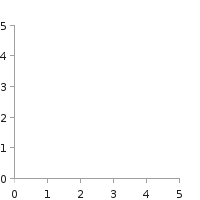
\includegraphics[width=0.3\textwidth]{numeric}}   
  \hspace{10pt}
  \subfloat[Numeric and categoric axis]{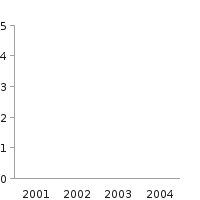
\includegraphics[width=0.3\textwidth]{numericcategoric}}
  \hspace{10pt}
  \subfloat[Two categoric axes]{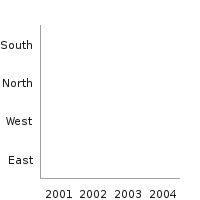
\includegraphics[width=0.3\textwidth]{categoriccategoric}}
  \caption{Different cartesian axis configurations}
  \label{cartesianaxes}
\end{figure}

A single polar axis determines the radius of the polar coordinate system. The axis is drawn in the horizontal position and duplicated in the vertical position. A visual representation of a polar coordinate system is shown in Figure \ref{polar}.

\begin{figure}[h!]
\centering
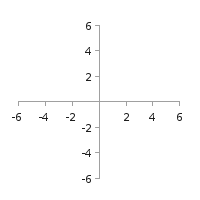
\includegraphics[width=.3\linewidth]{polar}
\caption{Polar coordinate system}
\label{polar}
\end{figure}

Both coordinate system do not draw a grid by default. Figure \ref{gridon} shows how grid lines are drawn when they are explicitly enabled. Note that the user can also choose to only draw the horizontal or vertical grid lines.

\begin{figure}[H]
	\centering
	\subfloat[Cartesian grid]{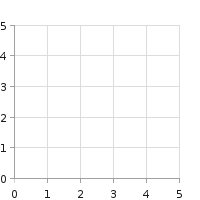
\includegraphics[width=0.3\textwidth]{numericgrid}}
	\subfloat[Polar grid]{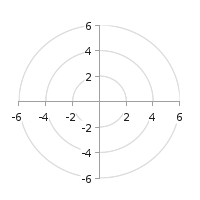
\includegraphics[width=0.3\textwidth]{polargrid}}
	\caption{Grid for cartesian and polar coordinate systems}
	\label{gridon}
\end{figure}

Because the canvas is a component, it has a minimum and a preferred size. The minimum size of the canvas is calculated by the width and height of the labels of its major tick marks, plus some additional spacing between the labels. A canvas' preferred size is the size it would like to have to optimally display data. This includes the minimum size multiplied by the preferred aspect ratio. A canvas' maximum size is a user defined setting of the maximum width and height the chart may attain. By default, a chart will try to use exactly the space given to it by its drawing area unless it violates either the minimum or maximum size. In this case the drawing area will be resized.

The aspect ratio defines the dimensions of a chart. The ratio itself is defined by either the horizontal and vertical axis or set by the user. If no ratio is given the library calculates it according to several heuristics aiming to reach an optimal $1:1$ ratio for most charts (other charts might have the golden ratio \cite{weisstein09, few04} set as default optimal value.) In order of importance, the heuristics are: 
\begin{itemize}
\item the resolution of the data (i.e. a maximum of one data point per screen pixel)
\item number and width of the axis labels
\item available space
\end{itemize}
The total size of a canvas is divided into two areas: a data area surrounded by padding necessary to contain all the labels. Figure \ref{outline} shows the data area marked by a red outline and the surrounding area marked with a blue outline.
\begin{figure}[h!]
\centering
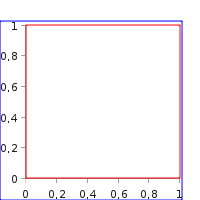
\includegraphics[width=.3\linewidth]{outline}
\caption{Outlines of the data area and surrounding area}
\label{outline}
\end{figure}
